
\subsection{Pre-fit screen: protocol, metrics, and real-series transfer}
\label{app:room}

\begin{figure*}[t]
\centering
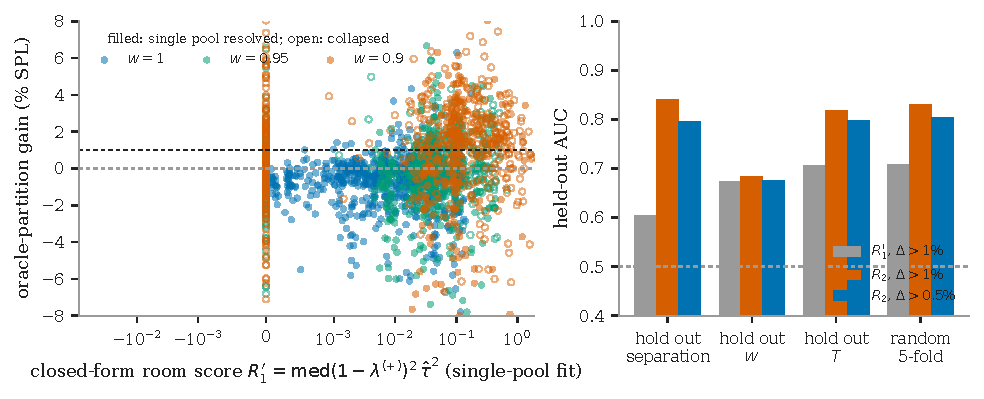
\includegraphics[width=0.96\textwidth]{figs/fig15_room_diagnostic.pdf}
\caption{\textbf{Screening for pooling room before any partition is
fitted.} Left: the closed-form score computed from the single-pool fit
against the oracle partition's realized gain on $2{,}700$ simulated
panels, colored by discount; open markers are panels whose single-pool
variance component collapsed. Right: held-out AUC for the event that the
oracle gain exceeds one percent (or half a percent), when whole
separation levels, discounts, or lengths are held out, or under random
folds; $R_1'$ is the closed-form score and $R_2$ a logistic screen on the
same fitting-window quantities.}
\label{fig:room}
\end{figure*}


\paragraph{Protocol.} The grid crosses separation $\{0,.25,.5,1,2\}$,
discount $\{1,.95,.90\}$, length $\{30,60,120\}$, occurrence mean
$\{.1,.25,.5\}$, items per group $\{20,60\}$, and balanced versus
$70/10/10/10$ group sizes, with four groups, $\tau^2=0.15$, $\sigma^2=1$,
occurrence separation scaled as $0.8\min(\mathrm{sep},1)$, five
replicates per cell, and seed 20260915. Per panel, only the single-pool
fit is used for features: median retained leverage on the size and
occurrence blocks, $\hat\tau^2$, the Beta concentration, the resolution
statistic, effective counts, and panel size. The target is the oracle
partition's paired pinball gain over the single pool (estimated
hyperparameters, true labels), which can be negative. The pre-registered
closed-form score $R_1$ used an unweighted mean of sampling variances
that is dominated by items whose discounted positive count approaches
zero; it has no screening power (AUC $0.45$--$0.64$) and is retained in
the released artifact. $R_1'$ replaces that term by the pool's own
weighted estimate $\hat\tau^2$; $R_2$ is a logistic regression on
$\log(1+\cdot)$ of the features, fitted on the training folds only. The
design, the amendments, and their order are recorded in
\texttt{docs/DESIGN\_room\_diagnostic.md}.

\begin{table}[t]
\centering
\caption{Held-out screening performance on the simulated grid for the
event that the oracle partition's gain exceeds one percent (base rate
$22\%$). Columns: AUC of the pre-registered $R_1$, of $R_1'$, and of the
logistic screen $R_2$ on all panels; the same for $R_1'$ and $R_2$ on the
panels whose single-pool variance component did not collapse; precision
and recall of $R_2$ at its best-$F_1$ threshold.}
\label{tab:room}
\small
\setlength{\tabcolsep}{3.5pt}
\begin{tabular}{lcccccc}
\toprule
 & \multicolumn{3}{c}{All panels} & \multicolumn{2}{c}{Resolved} & \\
\cmidrule(lr){2-4}\cmidrule(lr){5-6}
Held out & $R_1$ & $R_1'$ & $R_2$ & $R_1'$ & $R_2$ & $R_2$ P / R\\
\midrule
hold out a separation level & 0.45 & 0.60 & 0.84 & 0.72 & 0.85 & 0.54 / 0.77\\
hold out a discount & 0.64 & 0.67 & 0.68 & 0.66 & 0.68 & 0.51 / 0.49\\
hold out a length & 0.51 & 0.71 & 0.82 & 0.79 & 0.83 & 0.54 / 0.67\\
random 5-fold & 0.51 & 0.71 & 0.83 & 0.78 & 0.84 & 0.55 / 0.65\\
\bottomrule
\end{tabular}
\end{table}

\paragraph{Real-series transfer.} Online Retail, Carparts, and the
5{,}000-series M5 sample keep their zeros, noise, lengths, and scales; a
known partition is injected by multiplying every positive value of item
$i$ by $\exp(\delta_{g(i)})$ with symmetric offsets
$\{\pm0.5,\pm1.5\}\times\delta$, $\delta\in\{0,.25,.5,1,2\}$, over four
randomly assigned groups (three assignments), at the selected discount and
again at $w=0.90$. The oracle gain of the injected partition never exceeds
0.4\% on any panel: the single pool absorbs the injected
heterogeneity ($\hat\tau^2$ rises from $0.04$ to $5.1$ on Carparts as
$\delta$ goes from $0$ to $2$) and the median size-block credibility
rises toward one, so the items' own evidence, not the prior, carries the
forecast. $R_2$, fitted on the simulated grid and applied unchanged,
assigns every injected panel a probability below 0.17 of material
room (Figure~\ref{fig:room-transfer}). The transfer test therefore checks
the screen's rejections, not its detections; a real-series test of
detections would require panels whose items lack positive observations,
which is the short-history regime of Section~\ref{sec:pays}.

\begin{figure}[t]
\centering
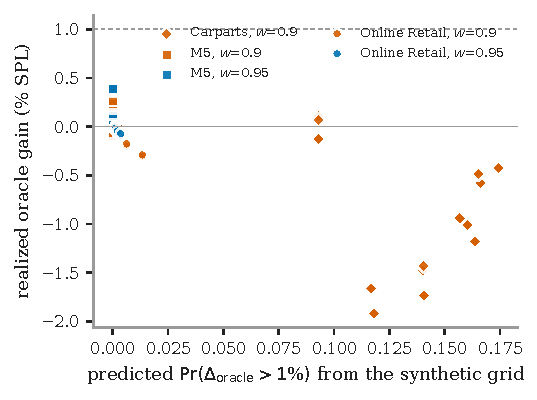
\includegraphics[width=0.9\linewidth]{figs/fig16_room_transfer.pdf}
\caption{Real-series transfer of the screen: predicted probability of
material room (from the simulated grid) against the realized oracle gain
of the injected partition, by panel and discount.}
\label{fig:room-transfer}
\end{figure}
